\documentclass[a4paper,11pt]{article}
\usepackage[a4paper, left=1.5cm, right=1.5cm, top=2.0cm, bottom=3.5cm, headsep=1.2cm]{geometry}
\usepackage{polski}
\usepackage{amssymb}
\usepackage[utf8]{inputenc}
\prefixing
\usepackage{latexsym}
\usepackage{graphicx}
\author{Klaudia Balcer}
\title{Raport 2}
\frenchspacing
\begin{document}
\maketitle
\tableofcontents
\pagebreak

\section{Zadanie 1}


\paragraph{a}

\paragraph{Wyestymowana macierz kowariancji:}

\left( \begin{array}{ccc}
46.229542 & -0.24821804 & -3.06203011 \\
-0.248218 & 0.06155249 & -0.02382592 \\
-3.062030 & -0.02382592 & 0.23084660 \\
\end{array} \right)

\paragraph{Wariancje} odpowiednio estymatorów $b_{0}, b_{1}, b_{2}$:

\begin{array}{ccc}
$Var(b_{0}) = 6.7985 ^{2} $ & $Var(b_{1}) = 0.2481 ^{2} $ & $Var(b_{2}) = 0.4804 ^{2}$ \\
\end{array}

Możemy zauważyć, że są one równe kolejnym wyrazom na przekątnej w macierzy kowariancji. Znając właściwości macierzy kowariancji tego też się spodziewaliśmy. 

\paragraph{b}

Będziemy testować, czy obie zmienne objaśniające nie mają wpływu na zmienną objaśnianą: 

$H_{0}: \quad \beta_{1} = \beta _{2} =  0$

$H_{1}: \quad \beta{1} \neq 0  \lor \beta_{2} \neq 0 $

Przez $M_{1}$ oznaczę model składający się tylko z Interceptu, przez $M_{2}$ - pełny model.



Wykorzystam statystykę deviance.%Pochodzi ona z rozkładu $\chi^{2}$ z $p-1$ stopniami swobody. 

$D(M_{2}) - D(M_{1})  =  39.74338 >  5.991465 = qchisq(0.95, 2)$

Czyli odrzucamy hipotezę zerową na rzecz alternatywnej, że co najmniej jedna ze zmiennym objaśniających ma wpływ na zmienną objaśnianą. 


\paragraph{c}

Będziemy testować, czy rozkład zmiennych jest zgodny z  założonym modelem. 


$H_{0}: \quad $ rozkład zmiennych jest zgodny z modelem

$H_{1}: \quad $ rozkład zmiennych nie jest zgodny z modelem


Wykorzystam statystykę Null deviance. Pochodzi ona z rozkładu $\chi^{2}$ z $n-p$ stopniami swobody. 

$D = 28.286 <  64.00111 = qchisq(0.95, 47)$

Czyli nie odrzucamy hipotezy zerowej, że dane są zgodne z założonym modelem. 

\paragraph{d}
\paragraph{
epsilon	} - dodatnia tolerancja konwergencji $\epsilon$; parametr decyduje o zatrzymaniu iteracji przy wyznaczaniu estymatora wektora $\beta$, gdy $ \frac{|dev - dev_{old}|}{|dev| + 0.1} < \epsilon$.

\begin{tabular}{r|c|cl|cl|cl}
epsilon & Fisher steps & intercept & p-value & numeraacy & p value & anxiety & p-value \\ \hline
defult: 1e-8 & 6 & 14.2386 & 0.03623 * & 0.5774  &  0.01995 * & -1.3841 & 0.00396 ** \\
1e-1 & 3 & 12.8901    & 0.012770 *  & 0.5376  & 0.007975 ** & -1.2640 & 0.000182 *** \\
1e-2 & 4 & 14.0925   & 0.02420 * &  0.5735 &  0.01430 * & -1.3713 & 0.00151 ** \\
1e-3 & 5 & 14.2368  &  0.03463 * &  0.5773 &  0.01930 * & -1.3839   & 0.00359 ** \\
1e-6 & 6 & 4.2386   &  0.03623 * & 0.5774& 0.01995 * & -1.3841  &  0.00396 ** \\
\end{tabular}

Tak jak się spodziewaliśmy - im mniejsza tolerancja, tym większa liczba iteracji, by dostać model, który jej nie będzie przekraczał.

Warto zwrócić uwagę, że estymatory współczynników regresji i ich p-wartości dla epsilon=1e-8 i epsilon=1e-6 wyszły identyczne. Dlaczego tak się stało? Dokładność do 1e-8 i do 1e-6 wymagała tej samej liczby iteracji, co za tym idzie - stworzyła identyczne modele (\textit{zmiana modelu} następuje po każdej kolejnej iteracji). 

Co ciekawe, dokładność przybliżeń nie powodowała pomniejszenia p-wartości. Idealnie dopasowane do danych równanie dostajemy, gdy n jest niewiększe niż p, jednak niekoniecznie będzie to dobry model. Mała próba może nie oddawać faktycznego stanu rzeczy, a model na niej oparty może dobrze poasować do danych, lecz słabo przystawać do rzeczywistości. 

\section{Zadanie 2}

W tej implementacji zadania użyłam modelu z interceptem (domyślna wartość w eRze -- i zazwyczaj podstaw do odrzucenia istotności interceptu szukamy w modelu, toteż w trakcie symulacji nie zakładałam znajomości sposobu generowania danych).

\paragraph{Macierz informacji Fishera} w puncie $\beta = (0, 3, 3, 3)'$:

\left(\begin{array}{cccc}
93.88248217 & 0.179727538  & -0.159775259 & 0.034361566 \\ 
0.17972754 & 0.223509010 & 0.009793625 & 0.015198422 \\
-0.15977526 & 0.009793625 & 0.237745775 & 0.002183475 \\
0.03436157 & 0.015198422 & 0.002183475 & 0.242009800 \\
\end{array}\right)

\paragraph{Macierz kowariancji} w puncie $\beta = (0, 3, 3, 3)'$:

\left(\begin{array}{cccc}
0.010681788 & -0.008850383 & 0.007552645 & -0.001028975 \\
-0.008850383 & 4.508547010 & -0.189098335 & -0.280177897 \\
0.007552645 & -0.189098335 & 4.219289342 & -0.027264345 \\
-0.001028975 & -0.280177897 & -0.027264345 & 4.150051563 \\
\end{array}\right)

\paragraph{a} Histogramy $\beta_{i}$  i deviance:

Wzbogaciłam histogramy o odpowiednie funkcje gęstości, ze średnią równą 3 i wariancją z odpowiednich wyrazów diagonali macierzy kowariancji. Zgodność empirycznego i teoretycznego rozkładu, jak na 500-elementową próbę, wydaje się być całkiem przyzowita.   

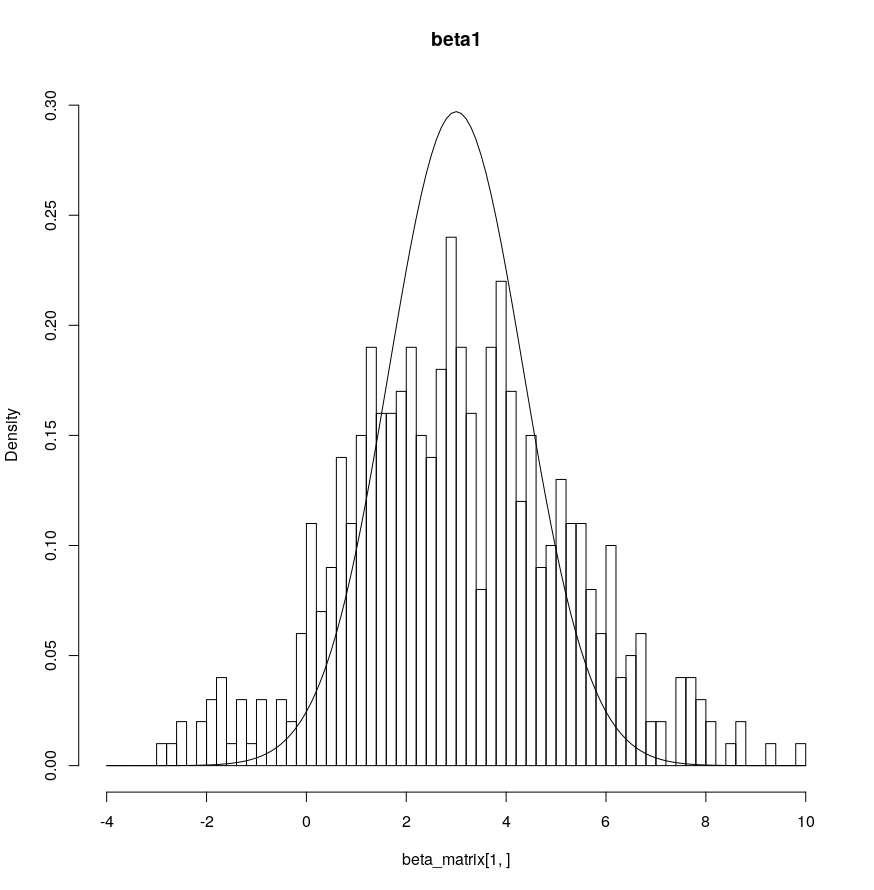
\includegraphics[scale=.35]{beta1.png} 
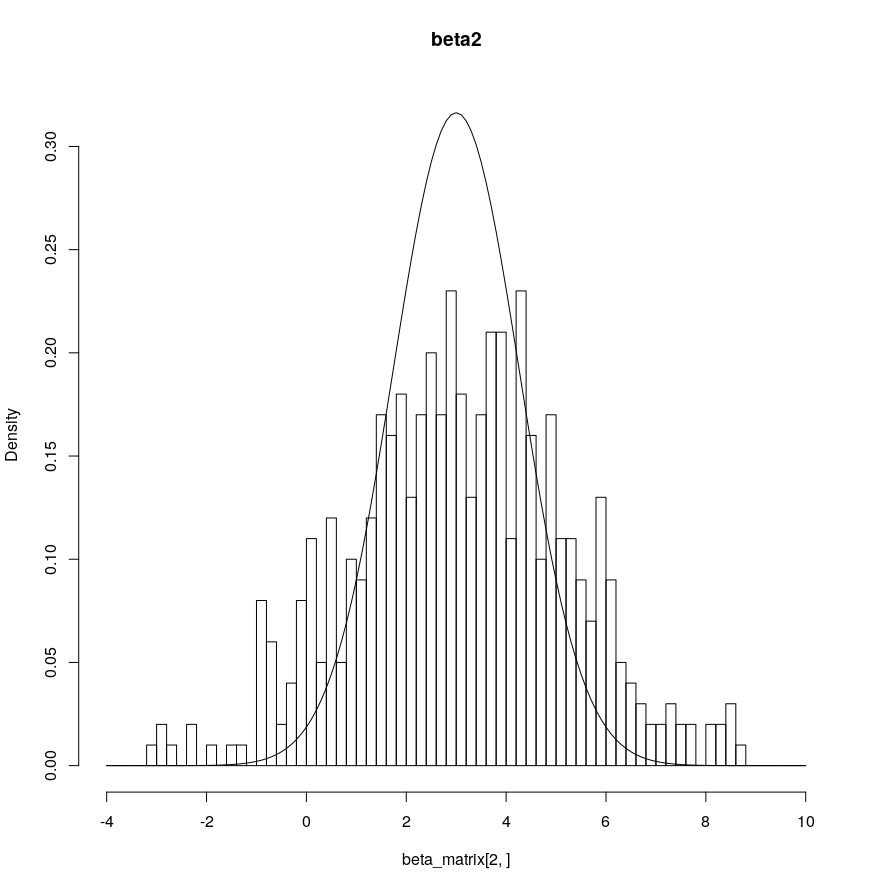
\includegraphics[scale=.335]{beta2.png}
 
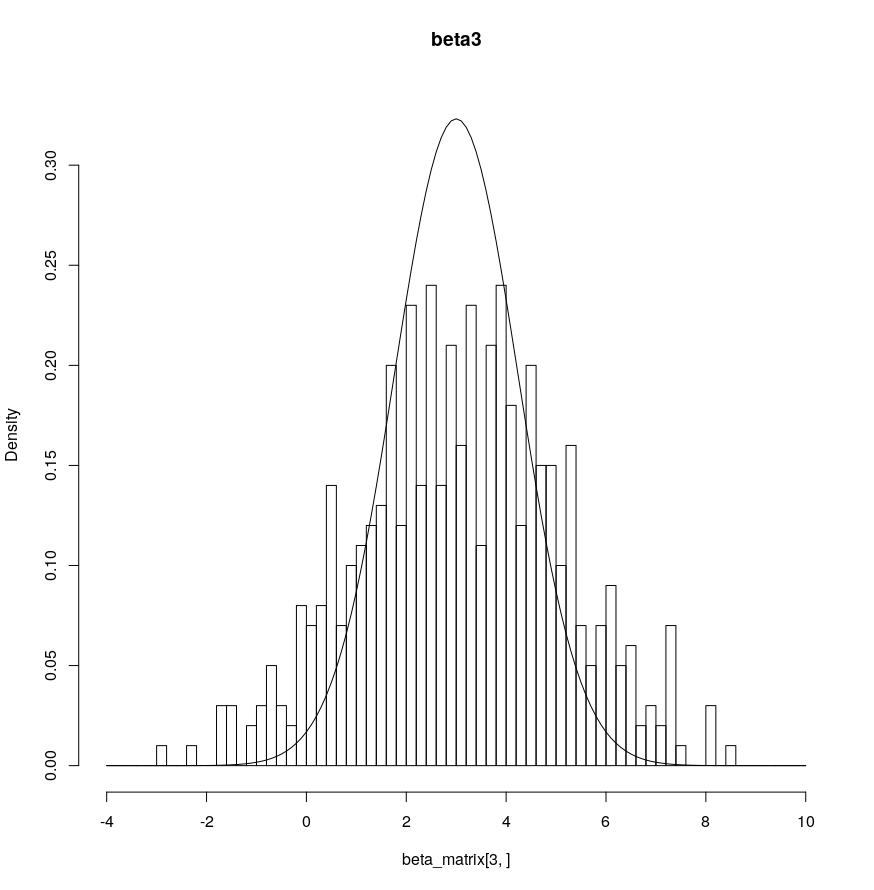
\includegraphics[scale=.35]{beta3.png} 
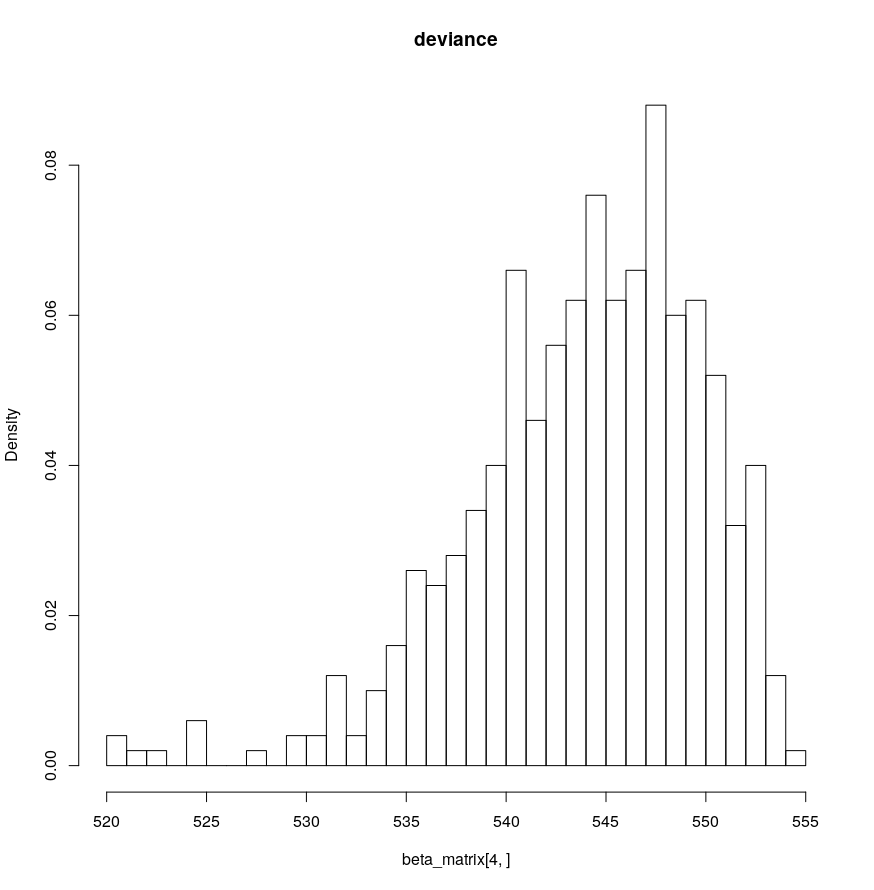
\includegraphics[scale=.35]{deviance.png} 

Dorysowywanie gęstości rozkładu $\chi^{2}$ uznałam za mylące, gdyż znacząca część nośnika przy tak wielu stopniach swobody jest dość rozległa i nie wpsółgra z uzyskanym histogramem (nie z powodu błędu, a właściwości rozkładu).

\paragraph{b} Obciążenia estymatorów $\widehat{\beta_{i}}$:

$

bias(b_{1}) =  0.03043006

bias(b_{2}) =  0.09967832

bias(b_{3}) =  0.08806881$

Obciżenia estymatorów powodują błędy względne rzędu $1-3\%$, błędy bezwzględne $< .1$. Jest to akceptowalne przy próbie wielkości 500.

\paragraph{c} 

By wyestymować macierz kowariancji utworzyłam model regresji logistycznej dla każdego z 500 wektorów odpowiedzi. Na tej podstawie za pomocą średniej próbkowej predykcyjnych wartości $p_{i}$ obliczyłam wyrazy na diagonali macierzy wagowej. 

Wyestymowana macierz kowariancji :

\left(\begin{array}{cccc}
0.010220217 & -0.01045698 & 0.005532991 & -0.002813691 \\
-0.010456976 & 4.35159156 & -0.136929781 & -0.213848453 \\
0.005532991 & -0.13692978 & 4.057571083 & 0.011764252 \\
-0.002813691 & -0.21384845 & 0.011764252 & 4.025174111 \\
\end{array}\right)

Jest ona stosunkowo bliska asymptotycznej macierzy kowariancji [przedstawionej na początku zadania]. 

\section{Zadanie 3}

Metoda implementacji poniższych zadań jest analogiczna do zadania 2., toteż skupię się  na omówieniu różnic miedzy wynikami. 

\paragraph{Macierz informacji Fishera} w puncie $\beta = (0, 3, 3, 3)'$:

\left(\begin{array}{cccc}
23.37740799 & 0.20012579 & 0.0730452891 & -0.1182702554 \\
0.20012579 & 0.19255387 & 0.0244930108 & 0.0108764657 \\
0.07304529 & 0.02449301 & 0.3058456161 & 0.0002064384 \\ 
-0.11827026 & 0.01087647 & 0.0002064384 & 0.1838149952 \\
\end{array}\right)

\paragraph{Macierz kowariancji} w puncie $\beta = (0, 3, 3, 3)'$:

\left(\begin{array}{cccc}
0.043345313 & -0.04592748 & -0.006694844 & 0.03061432 \\
-0.045927480 & 5.31318510 & -0.414294670 & -0.34347037 \\
-0.006694844 & -0.41429467 & 3.304389183 & 0.01649543 \\
0.030614325 & -0.34347037 & 0.016495434 & 5.48025530 \\
\end{array}\right)

\paragraph{a} Histogramy $\beta_{i}$ i deviance:

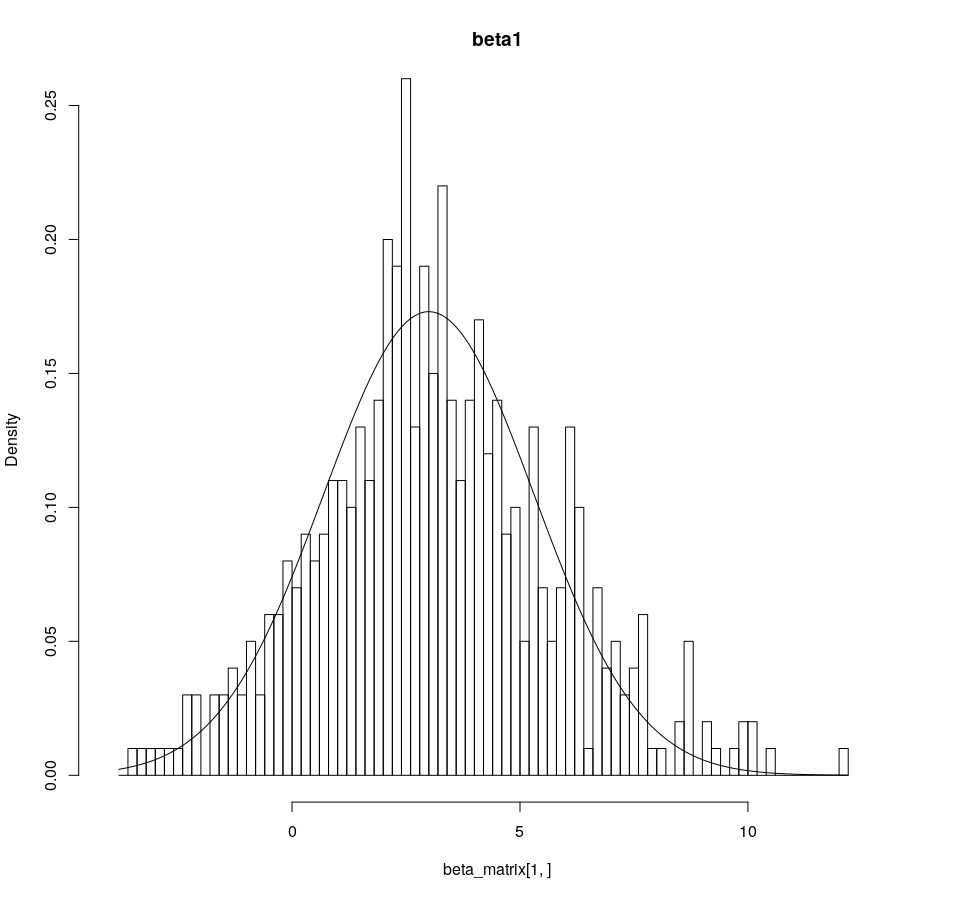
\includegraphics[scale=.35]{beta1_3.png} 
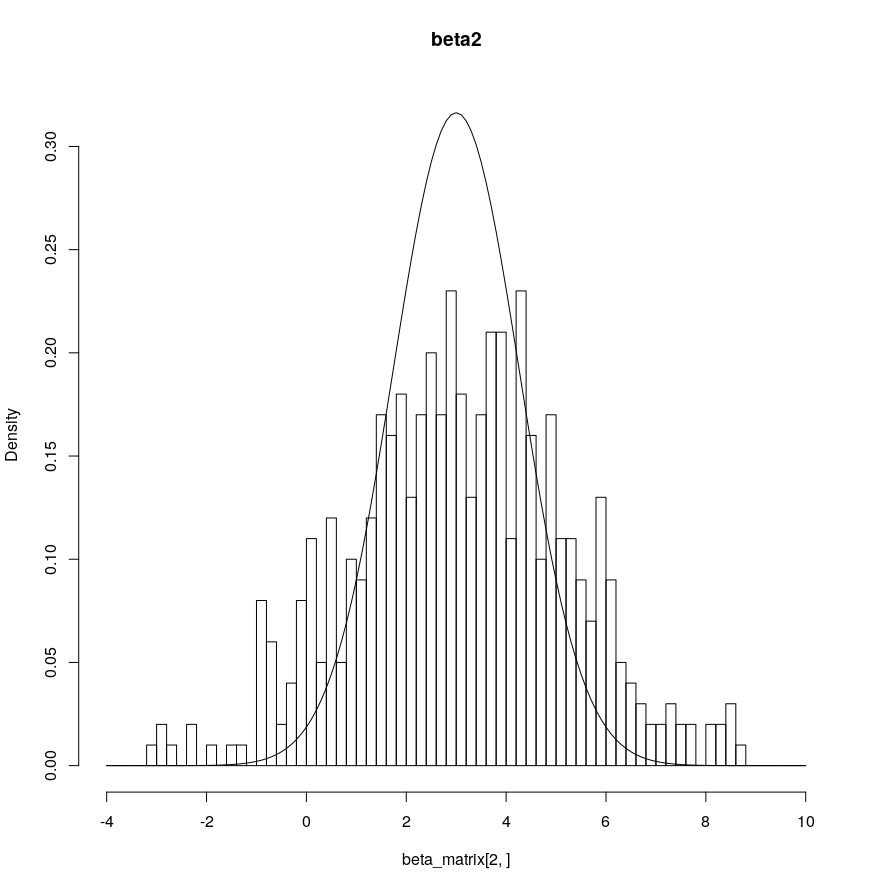
\includegraphics[scale=.35]{beta2.png} 

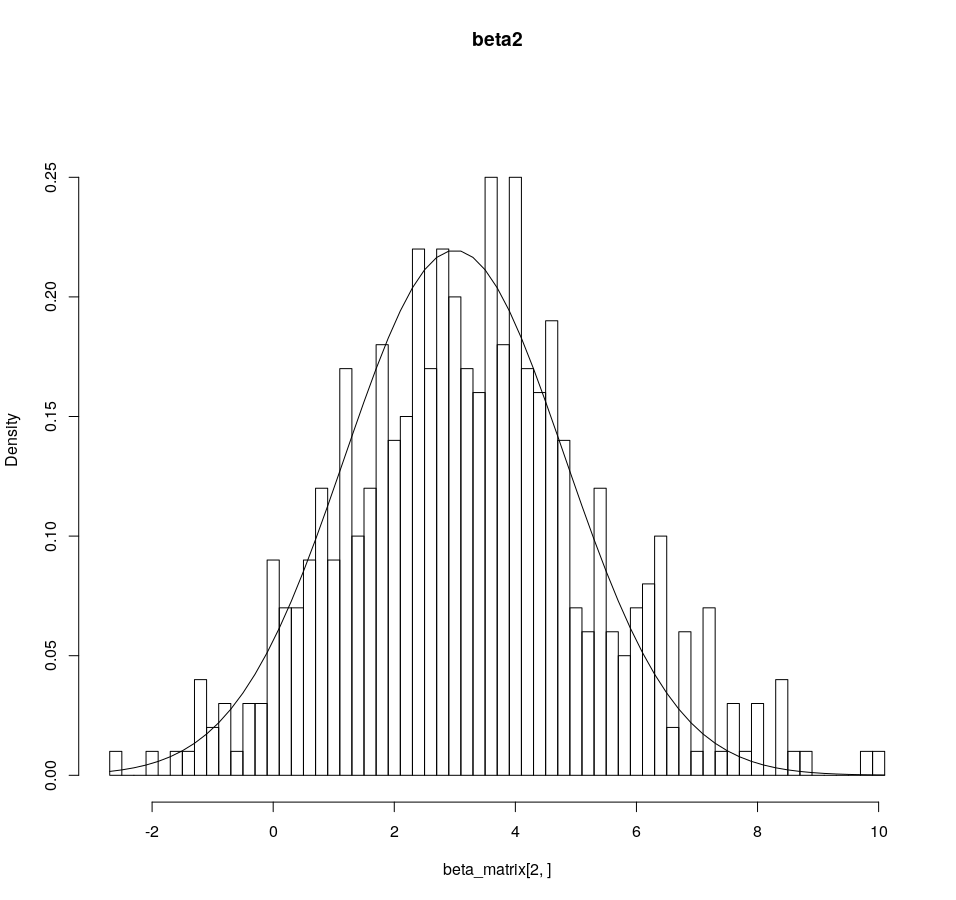
\includegraphics[scale=.35]{beta2_3.png} 
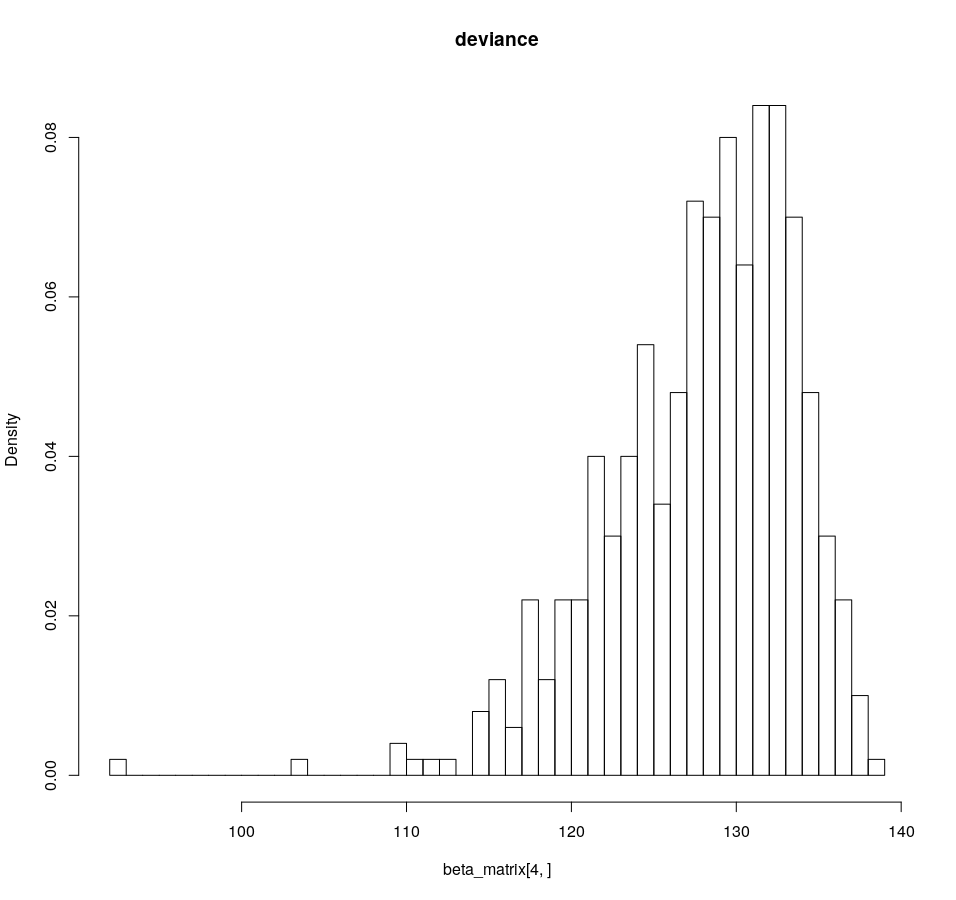
\includegraphics[scale=.35]{deviance_3.png} 

Dopasowanie histogramów do asymptotycznych gęstości jest na pdoobnym poziomie, co w zadaniu 2. 

\paragraph{b} Obciążenia estymatorów $\widehat{\beta_{i}}$:

$

bias(b_{1}) = 0.135795

bias(b_{2}) = 0.263659

bias(b_{3}) = 0.1375891 $

Zmiejszenie n powoduje zwiększenie obciążenia estymatorów $\beta$. Dla $n=100$ obciążenia te dają błąd względny rzędu $4-9/%$ i błąd bezwzględny w okolicach 0.2 --  czyli około 20-krotnie wyższy niż dla$n=400$. 


\paragraph{c} 

Wyestymowana macierz kowariancji :

\left(\begin{array}{cccc}
0.04372489 & -0.05334905 & -0.01142417 & 0.02605673 \\
-0.05334905 & 5.50634710 & -0.11490675 & -0.24234393 \\
-0.01142417 & -0.11490675 & 3.53382363 & 0.25994266 \\
0.02605673 & -0.24234393 & 0.25994266 & 5.73923818 \\
\end{array}\right)

Błędy względne estymatorów wariancji estymatorów $\beta$:
\begin{center} \begin{tabular}{|c|c|c|c|}
n & $Var(b_{1})$ & $Var(b_{2})$ & $Var(b_{3})$  \\  \hline
n = 400 & 0.03481287 & 0.03832832 & 0.03009058 \\
n = 100 &  0.036355216 & 0.069433239 & 0.047257447 \\
\end{tabular} \end{center}

Błędy bezwzględne estymatorów wariancji estymatorów $\beta$:

\begin{center} \begin{tabular}{|c|c|c|c|}
n & $Var(b_{1})$ & $Var(b_{2})$ & $Var(b_{3})$  \\ \hline 
n = 400 & 0.1569554515 & 0.1617182589 & 0.1248774519 \\
n = 100 &  0.1931619931 & 0.2294344443 & 0.2589828765 \\
\end{tabular} \end{center}

Asymptotyczna wariancja estymatorów $\beta$ jest większa dla n=100, ponadto estymacja tej wariancji daje większe błędy względne i bezwzględne. Nie sa to bardzo znaczące różnice, niemniej widocznym jest, że mniejsze n daje słabszą estymację współczynników regresji logistycznej. 

\section{Zadanie 4}

W tym zadaniu zobaczymy zachowanie modelu, gdy zmienne objaśniające są ze sobą zależne (macierz sigma ma niezerowe wyrazy poza przekątną).

\subsection{n=400}


\paragraph{Macierz informacji Fishera} w puncie $\beta = (0, 3, 3, 3)'$:

\left(\begin{array}{cccc}
90.736208 & -10.20158  & -9.740752 &  -7.222384 \\
-10.201579 & 86.30609  & 25.991116 &  21.346668 \\ 
-9.740752  &  25.99112  & 96.803699  & 25.270194 \\
-7.222384  &  21.34667  & 25.270194  & 85.483793 \\
\end{array}\right)

\paragraph{Macierz kowariancji} w puncie $\beta = (0, 3, 3, 3)'$:

\left(\begin{array}{cccc}
0.0112500109  &  0.000986794  &  0.0007404115 &   0.0004852007\\
0.0009867940  &  0.013134626 &  -0.0028096292  & -0.0023659878\\
0.0007404115 &  -0.002809629  &  0.0118760286  & -0.0027465532\\
0.0004852007 &  -0.002365988 &  -0.0027465532   & 0.0131418618\\
\end{array}\right)

Wyrazy macierzy kowariancji są istotnie mniejsze niż w przypadku niezależnych zmiennych objaśniających.

\paragraph{a} Histogramy $\beta_{i}$ i deviance:

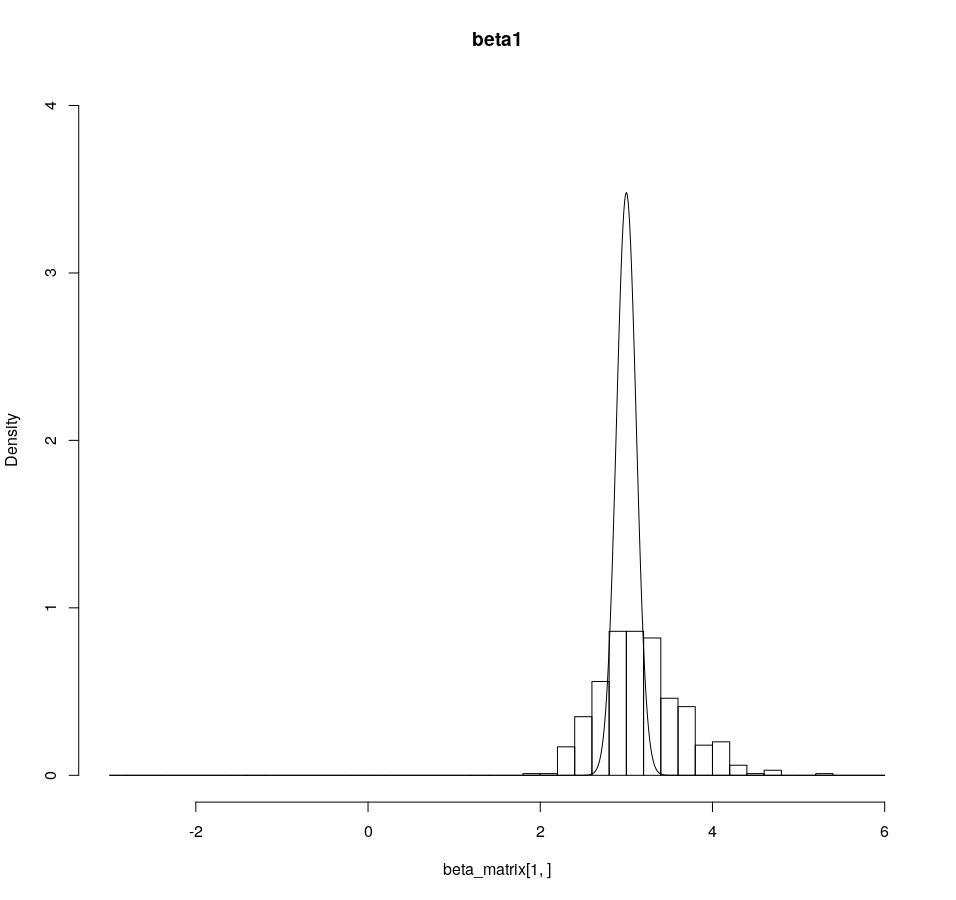
\includegraphics[scale=.35]{beta42_1.png} 
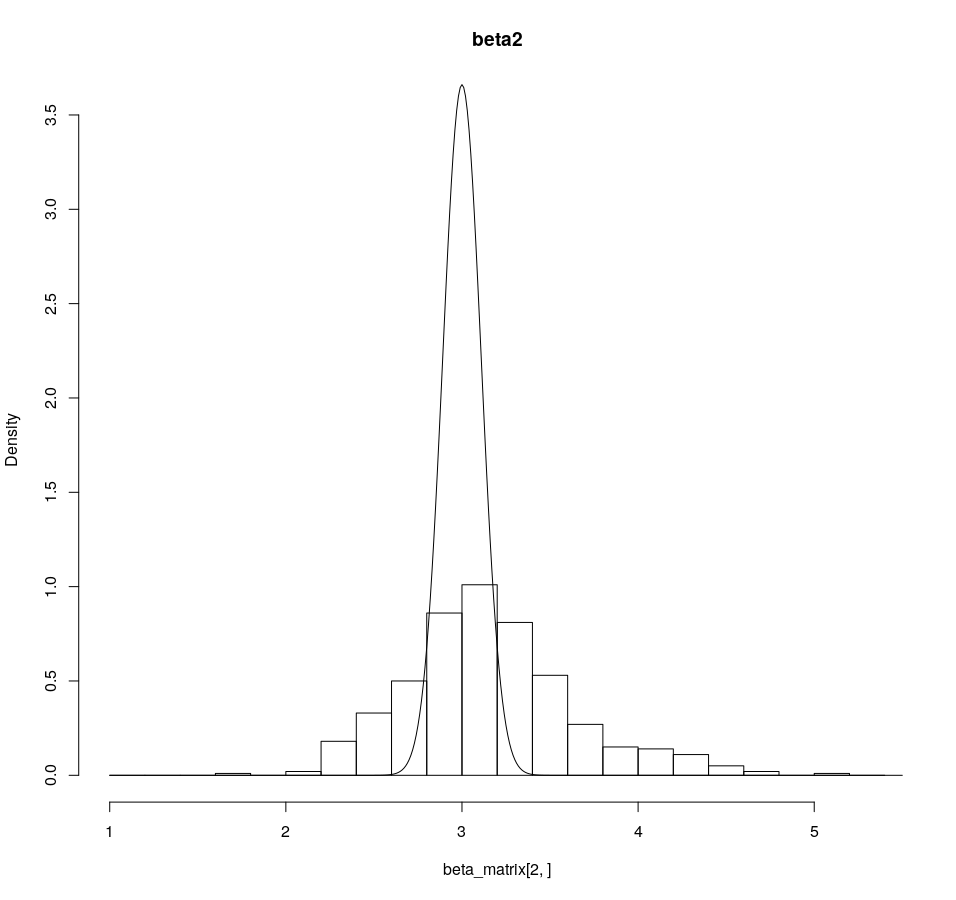
\includegraphics[scale=.35]{beta42_2.png} 
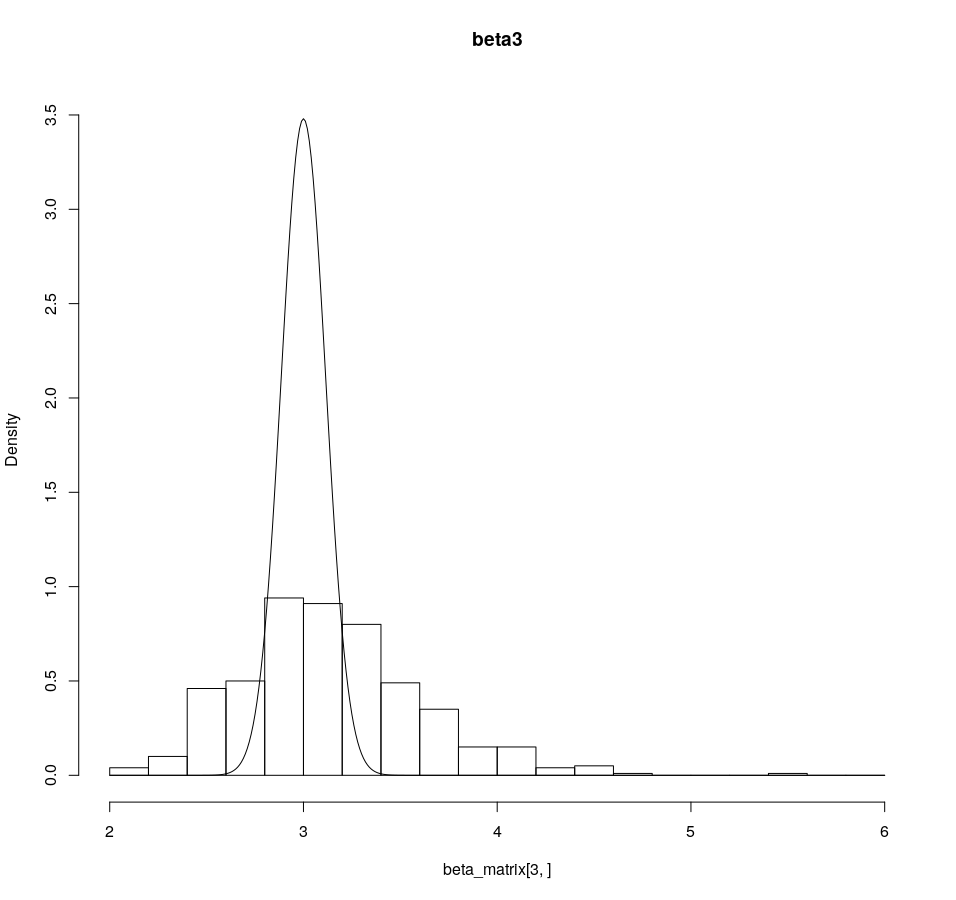
\includegraphics[scale=.35]{beta42_3.png} 
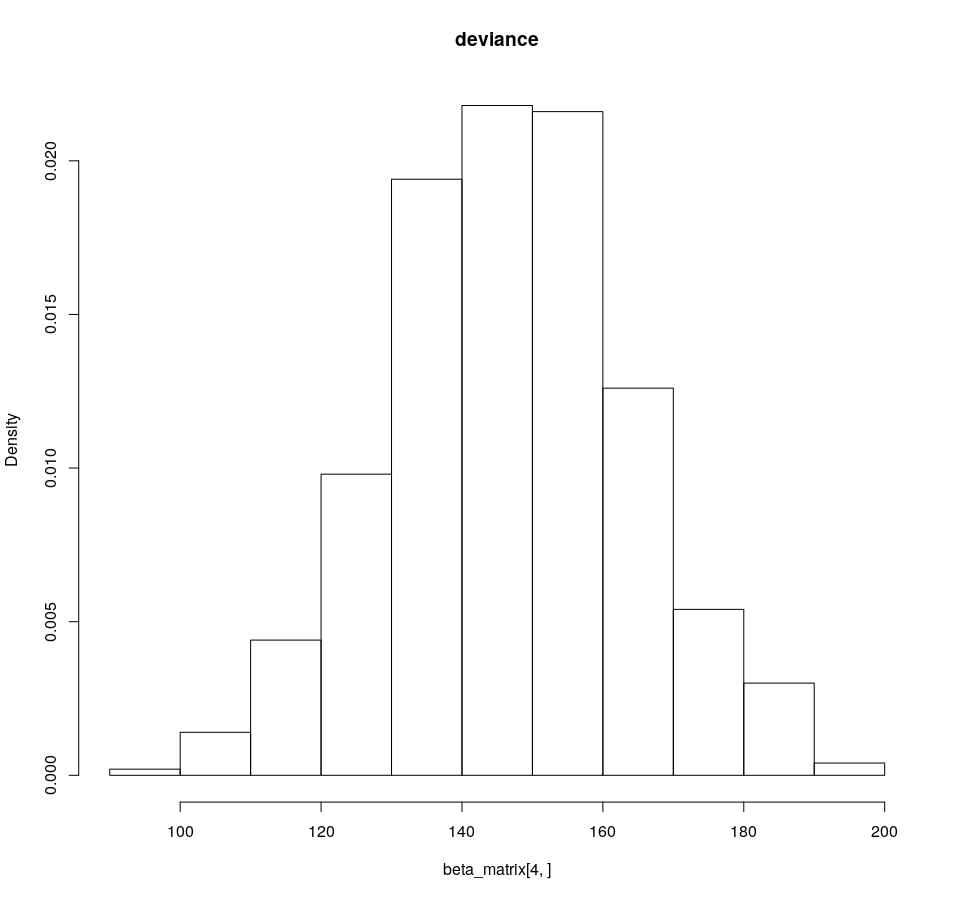
\includegraphics[scale=.35]{deviance_42.png} 

Histogramy są znacznie dalsze asymptotycznym rozkładom niż w poprzednich zadaniach. 

\paragraph{b} Obciążenia estymatorów $\widehat{\beta_{i}}$:

$

bias(b_{1}) = 0.1676119

bias(b_{2}) = 0.1608707

bias(b_{3}) = 0.1424548 $

Obciążenie estymatorów współczynników regresji logistycznej przy zależnych zmiennych objaśniających dla 400 obserwacji jest porównywalne z wynikami dla niezależnych X i n=100. 


\paragraph{c} 

Wyestymowana macierz kowariancji :

\left(\begin{array}{cccc}
0.0449141240  & -0.002893998  & -0.0003988058 &  -0.002127385\\
-0.0028939978  &  0.207041169  &  0.1305549846  &  0.130098523\\
-0.0003988058  &  0.130554985 &   0.1808843803   & 0.129969260\\
-0.0021273853  &  0.130098523 &   0.1299692596   & 0.190232724\\
\end{array}\right)

Ze względu na bardzo małe asymptotyczne wariancje $b_{i}$ błąd względny przy estymacji macierzy kowariancji jest duży. Błąd względny jest jednak na poziomie 0.15 -- porównywalnie z wynikami zadania 3. 


Przy dużej liczbie obserwacji zależność zmiennych objaśniających nie psuje wyników. 

\subsection{n=100}


\paragraph{Macierz informacji Fishera} w puncie $\beta = (0, 3, 3, 3)'$:

\left(\begin{array}{cccc}
22.740830 & -2.074993 & -3.256282 & -3.941950 \\
-2.074993 & 21.671551 & 2.760231 & 2.029436 \\ 
-3.256282 & 2.760231 & 22.268942 & 8.518226 \\
-3.941950 & 2.029436 & 8.518226 & 20.310731 \\
\end{array}\right)

\paragraph{Macierz kowariancji} w puncie $\beta = (0, 3, 3, 3)'$:

\left(\begin{array}{cccc}
0.046019148 & 0.003282473 & 0.003610543 & 0.007089267 \\
0.003282473 & 0.047240237 & -0.004542262 & -0.002178143 \\ 
0.003610543 & -0.004542262 & 0.054259507 & -0.021601582 \\
0.007089267 & -0.002178143 & -0.021601582 & 0.059888198 \\
\end{array}\right)

\paragraph{a} Histogramy $\beta_{i}$  i deviance:

Przed podaniem histogramów pokażę, jak różnie zostały wyestymowane b dla kolejnych wektorów odpowiedzi, podając poniżej najmniejsze i największe wyniki w modelach przy 100 obserwacjach i trzech zależnych zmiennych objaśniających:
\begin{center}
\begin{tabular}{c|c|c}
 & min & maks \\
$\beta_{1}$ & 1.557905  & 1811.040945 \\
$\beta_{2}$ &  1.470084  & 1467.833113 \\ 
$\beta_{3}$  & 1.399734  & 1360.790948 \\
deviance  & 6.791038e-08 &  5.628472e+01 \\
\end{tabular}
\end{center}


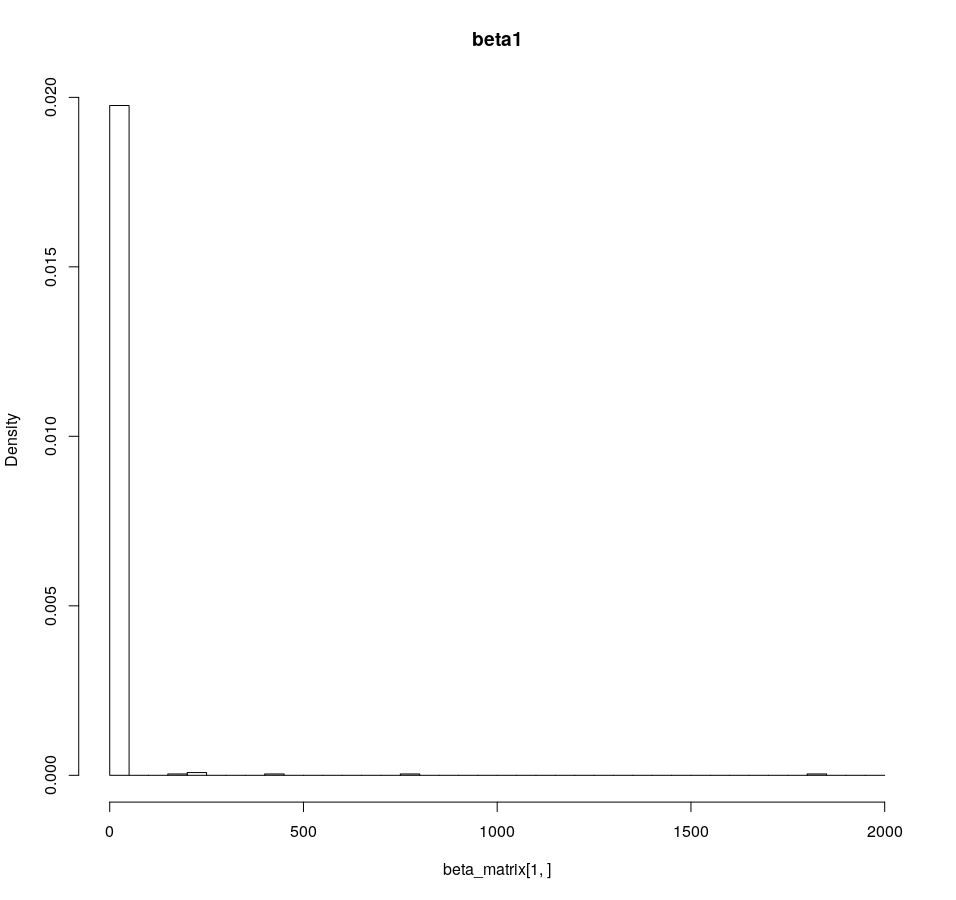
\includegraphics[scale=.35]{beta43_1.png} 
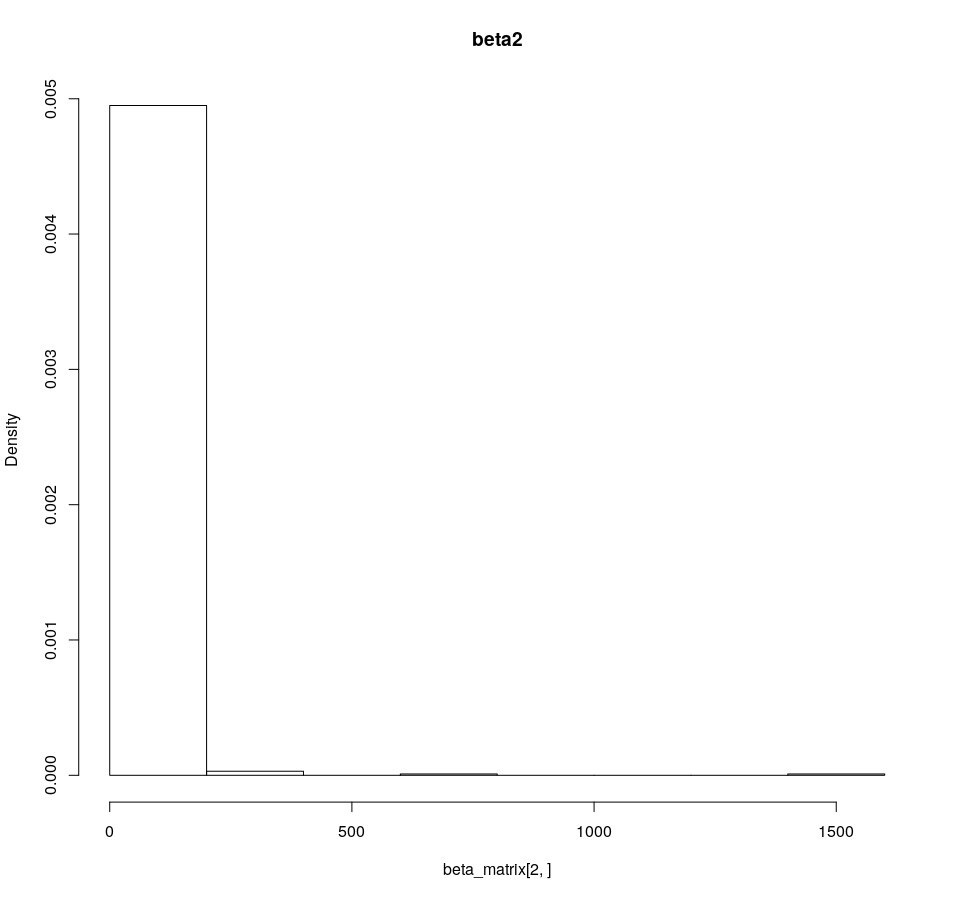
\includegraphics[scale=.35]{beta43_2.png} 
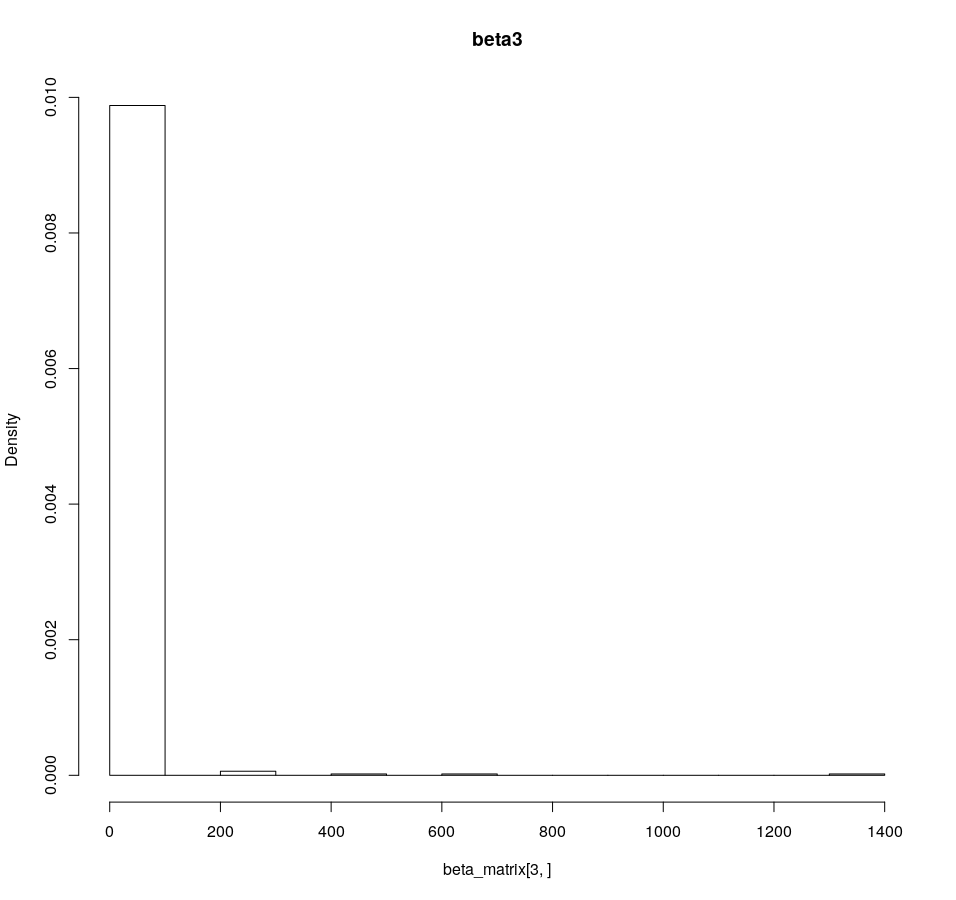
\includegraphics[scale=.35]{beta43_3.png} 
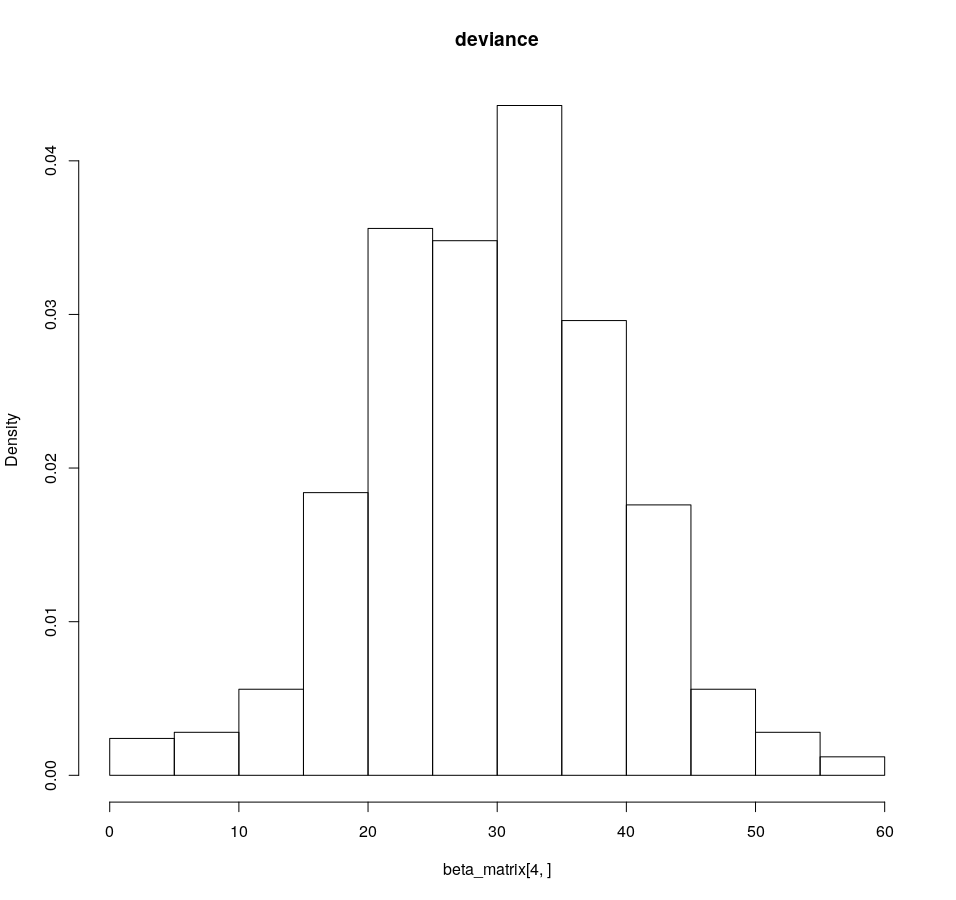
\includegraphics[scale=.35]{deviance_43.png} 

Patrząc na histogramy nie jesteśmy w stanie wychwycić ewentualnej obecności obserwacji wpływowych, gdyż mamy pewną liczbę obserwacji znacznie odstających i zaburzających obraz rozkladu b. Co wpłynęło na znacznie większe niż wcześniej obciążenia i błąd w estymacji macierzy kowariancji. 

\paragraph{b} Obciążenia estymatorów $\widehat{\beta_{i}}$:

$

bias(b_{1}) = 8.310843

bias(b_{2}) = 7.262548

bias(b_{3}) = 7.435932 $

Obciążenie jest ogromne. 

\paragraph{c} 

Wyestymowana macierz kowariancji :

\left(\begin{array}{cccc}
1.667433 & -7.14772 & -5.963199 & -5.842985 \\
-7.147720 & 51.05578 & 44.075614 & 43.243116 \\
-5.963199 & 44.07561 & 39.700476 & 37.775696 \\
-5.842985 & 43.24312 & 37.775696 & 37.575716 \\
\end{array}\right)

Wyestymowana macierz absolutnie nie przystaje do macierzy asymptotycznej. 

\subsection{Wnioski}

Dla odpowiednio dużej liczby obserwacji n estymacja wpsółczynników regresji logistycznej daje przyzwoite wyniki. Zmniejszenie n powoduje jednak gwałtowne i znaczne zaburzenia.  Zmiany wiarygodności wyników są znacznie większe niż w przypadku niezależnych zmiennych objaśniających. Wymaga to znacznie uważniejszego podejścia  (być może eliminując outlierów uzyskalibyśmy bardziej wiarygodne wyniki). 

\subsection{n=100 - symulacja z odrzuceniem outlierów}

Postanowiłam wcielić wnioski w życie i przeprowadzić symulację z wykluczeniem do $6/%$ odstających obserwacji (zrobiłam to metodą analogiczną do Bonferroniego i podzieliłam budżet błędu na po $2/%$ dla każdego współczynnika regresji). Odstawanie oceniałam na podstawie oddalenia od mediany (średnia byłaby niemiarodajna, gdyż outliery znacznie ją zawyżały).

Zmiana w implementacji przedstawiała się następująco:

\begin{verbatim}
beta_matrix <- sapply(seq(500), function(i){
  model <- glm(Y500[,i]~X[,1]+X[,2]+X[,3], family = "binomial") #intercept = FALSE
  c(model$coefficients[2], model$coefficients[3], model$coefficients[4], 
  	model$deviance, model$coefficients[1])})
  	
mediana <- sapply(seq(5), function(i){median(beta_matrix[i, ])})
err <- sapply(seq(5), function(i){beta_matrix[i, ]-mediana})
to_be_deleted <- sort(c(which(err[,1]>quantile(err[,1], .98)), 
						which(err[,2]>quantile(err[,2], .98)), 
						which(err[,3]>quantile(err[,3], .98))))
res <- c()
for(i in 1:500){
  control <- TRUE
  for(j in 1:length(to_be_deleted)){
    if(i==to_be_deleted[j]){
      control <- FALSE
    }
  }
  if(control){res <- c(res, i)}
}
beta_matrix_improved <- beta_matrix[, res]
\end{verbatim}

Użyłam nieefektywnej metody z pętlami w R, niemniej jednak nie każda iteracja miała coś zwracać, toteż użycie sapply w tym algorytmie nie może mieć miejsca, a taki właśnie sposób postępowania wydał mi się najbardziej przystępny. 

\paragraph{a} Histogramy $\beta_{i}$  i deviance:

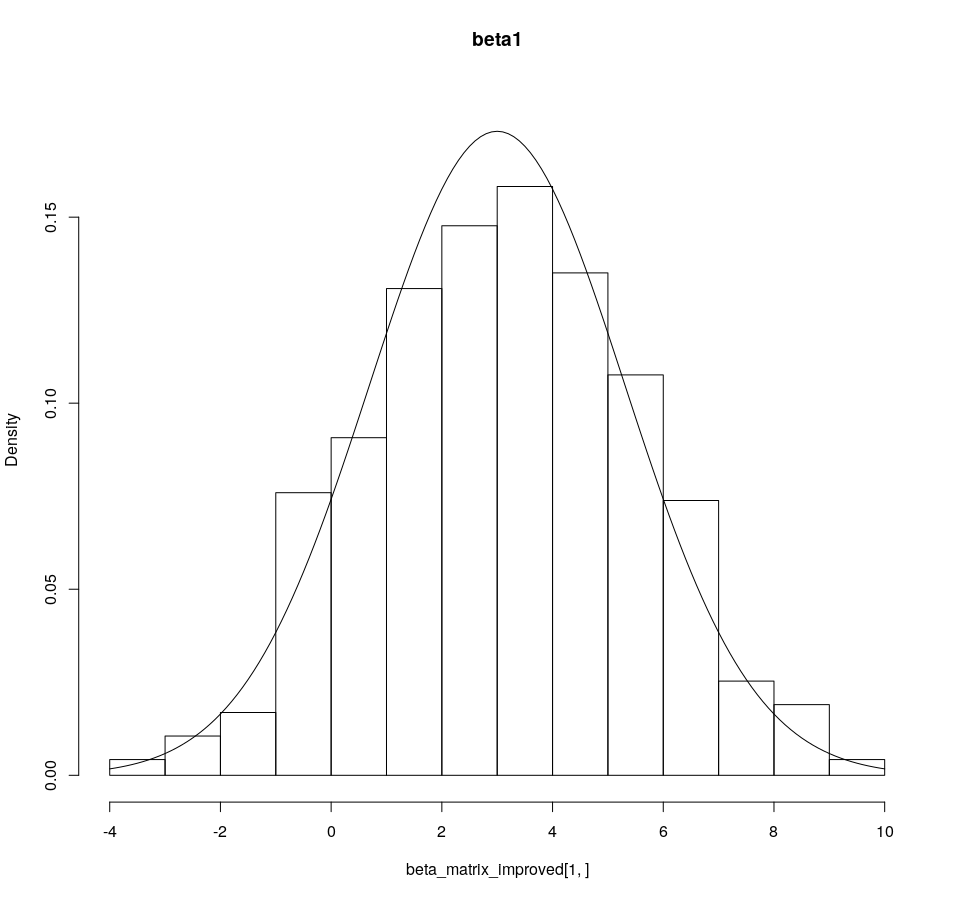
\includegraphics[scale=.35]{e1.png} 
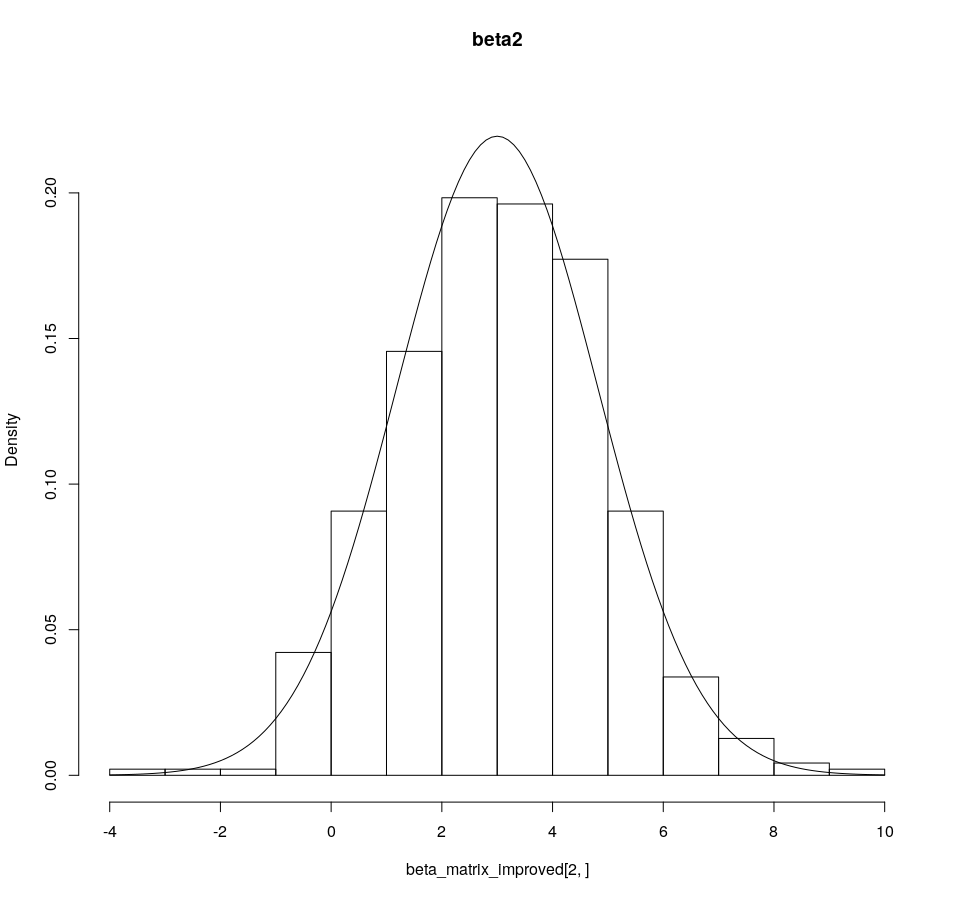
\includegraphics[scale=.35]{e2.png} 
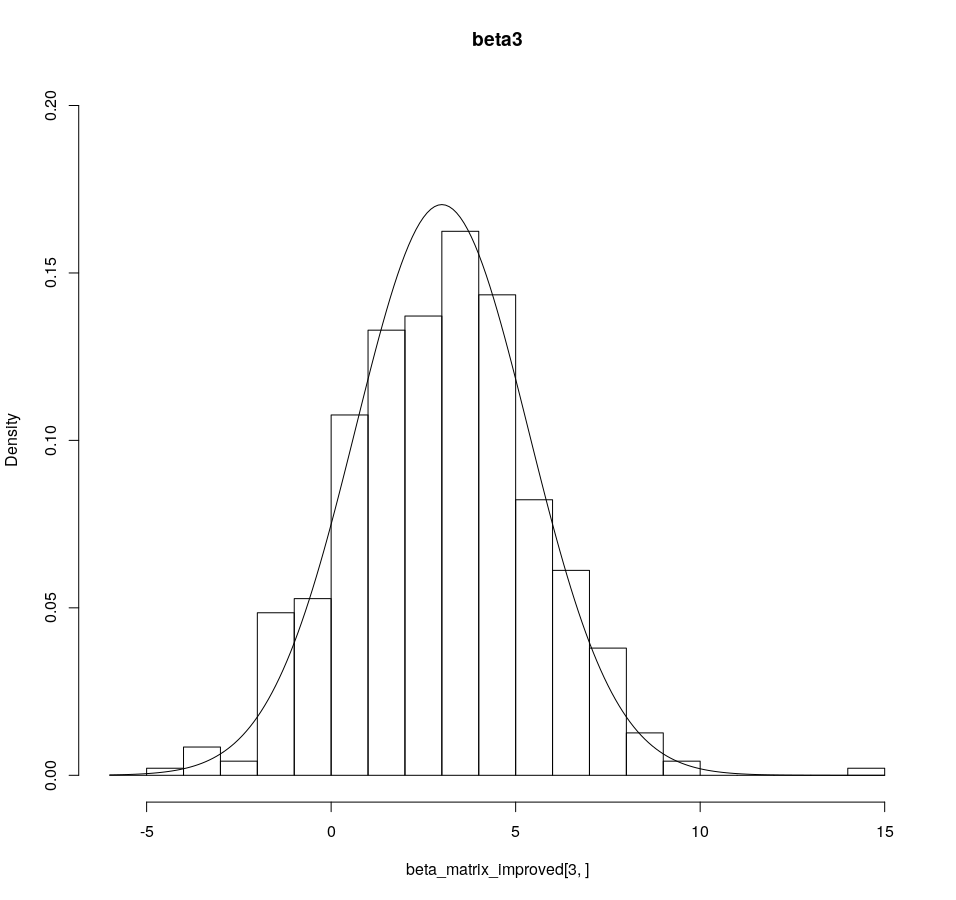
\includegraphics[scale=.35]{e3.png} 
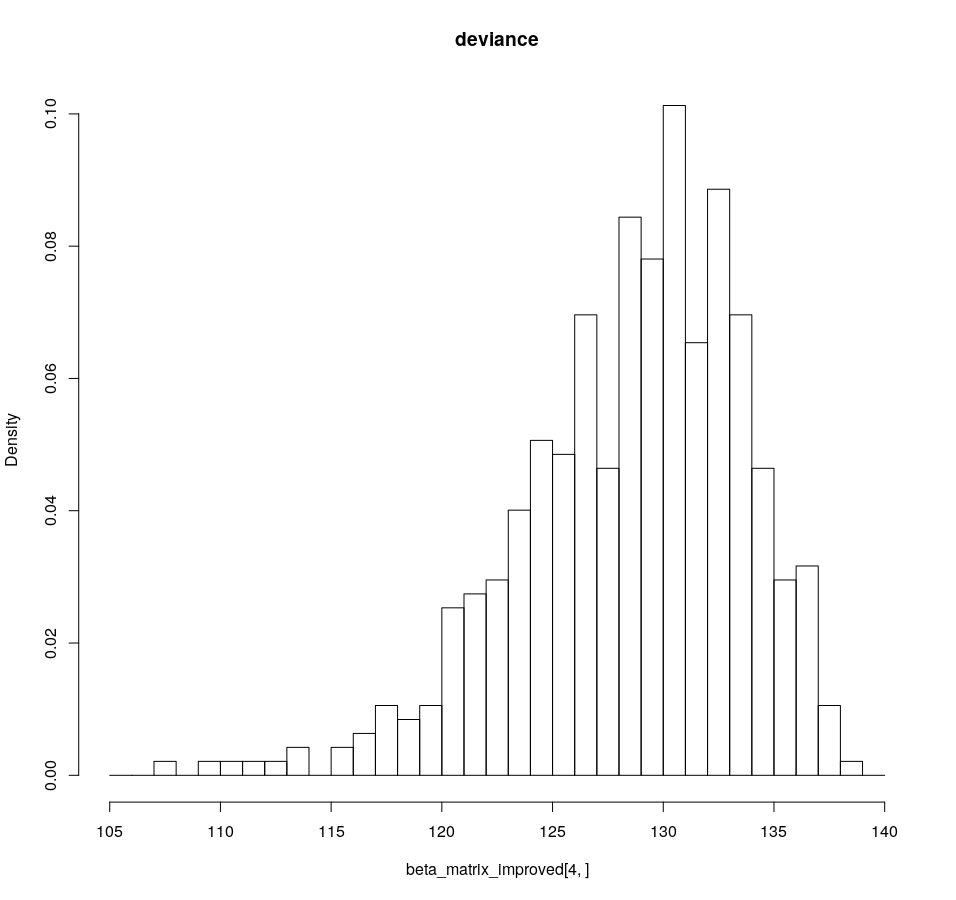
\includegraphics[scale=.35]{e4.png} 

Widzimy, że tylko dla $b_{3}$ odrzucenie $2/%$ obserwacji odstających pozostawiło outliera. Niemniej jednak jest on oddalony od wartości oczekiwanej estymatora dużo mniej niż to można było zauważyć w poprzedniej implementacji. 


\paragraph{b} Obciążenia estymatorów $\widehat{\beta_{i}}$:

$
bias(b_{1}) = 0.2378524

bias(b_{2}) = 0.2077744

bias(b_{3}) = 0.06367604$

Po odrzuceniu obserwacji odstających, obciążenie estymatora współczynników regresji logistycznej wróciło do stanu akceptowalnego.

\paragraph{c} 

Wyestymowana macierz kowariancji:


\left(\begin{array}{cccc}
 0.04370757 & -0.05367444 & -0.01181205 &  0.02582357 \\
-0.05367444 &  5.51410242 & -0.11219826 & -0.24211123 \\ 
-0.01181205 & -0.11219826 &  3.52694892 &  0.24985040 \\
 0.02582357 & -0.24211123 &  0.24985040 &  5.72262367 \\
 \end{array}\right)
 
 Macierz kowariancji estymatorów różni się znacznie od asymptotycznej, niemniej jednak i tutaj wyrzucenie outlierów zmniejszyło błąd. 

\section{Zadanie 5}

\subsection{n=400}


\paragraph{Macierz informacji Fishera} w puncie $\beta = (0, 3, 3, 3, 0, 0, 0, \ldots)'$:

\left(\begin{array}{ccccccc}
93.88248217 &   0.179727538 &  -0.159775259  & 0.034361566  & -0.385143555  &  0.179330740 & \ldots \\
0.17972754  &  0.223509010  &  0.009793625 &  0.015198422 &  -0.015505792  &  0.007263230 & \ldots \\
-0.15977526  &  0.009793625  &  0.237745775 &  0.002183475  &  0.010042652  &  0.011403094 & \ldots \\
0.03436157  &  0.015198422  &  0.002183475  & 0.242009800   & 0.005705871  &  0.014241778 & \ldots \\
-0.38514356 &  -0.015505792  &  0.010042652  & 0.005705871  &  0.223683084 &  -0.009582992 & \ldots \\
 0.17933074  &  0.007263230  &  0.011403094  & 0.014241778 &  -0.009582992  &  0.256719151 & \ldots \\
 \dots & \dots & \dots & \dots & \dots & \dots & \ddots \\
\end{array}\right)

\paragraph{Macierz kowariancji} w puncie $\beta = (0, 3, 3, 3, 0, 0, 0, \ldots)'$:

\left(\begin{array}{ccccccc}
0.010973611 &  -0.006128395  &  0.006483011  &  0.001019718  &  0.01824566 &  -0.008019834 & \ldots \\
-0.006128395  &  4.779311111  & -0.242867545 &  -0.299172835  &  0.32174181 &  -0.068019713 & \ldots \\
0.006483011  & -0.242867545  &  4.376532047  & -0.046809947  & -0.22782025  & -0.246101675 & \ldots \\
0.001019718  & -0.299172835  & -0.046809947   & 4.384208925 &  -0.10465954  & -0.235519218 & \ldots \\
0.018245656  &  0.321741814 &  -0.227820255  & -0.104659539  &  4.69594841  &  0.282330614 & \ldots \\
-0.008019834  & -0.068019713 &  -0.246101675  & -0.235519218 &   0.28233061  &  4.166461237 & \ldots \\
 \dots & \dots & \dots & \dots & \dots & \dots & \ddots \\
\end{array}\right)

\paragraph{a} Histogramy $\beta_{1, 2, 3}$ i deviance:

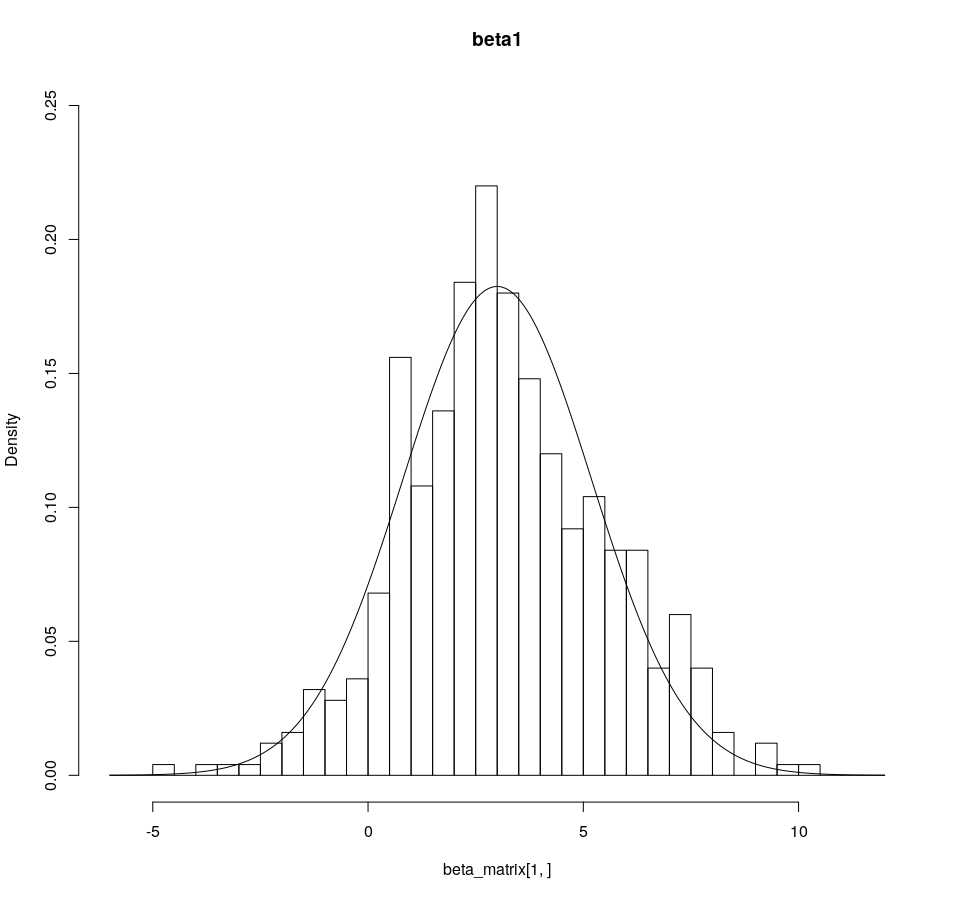
\includegraphics[scale=.35]{521.png} 
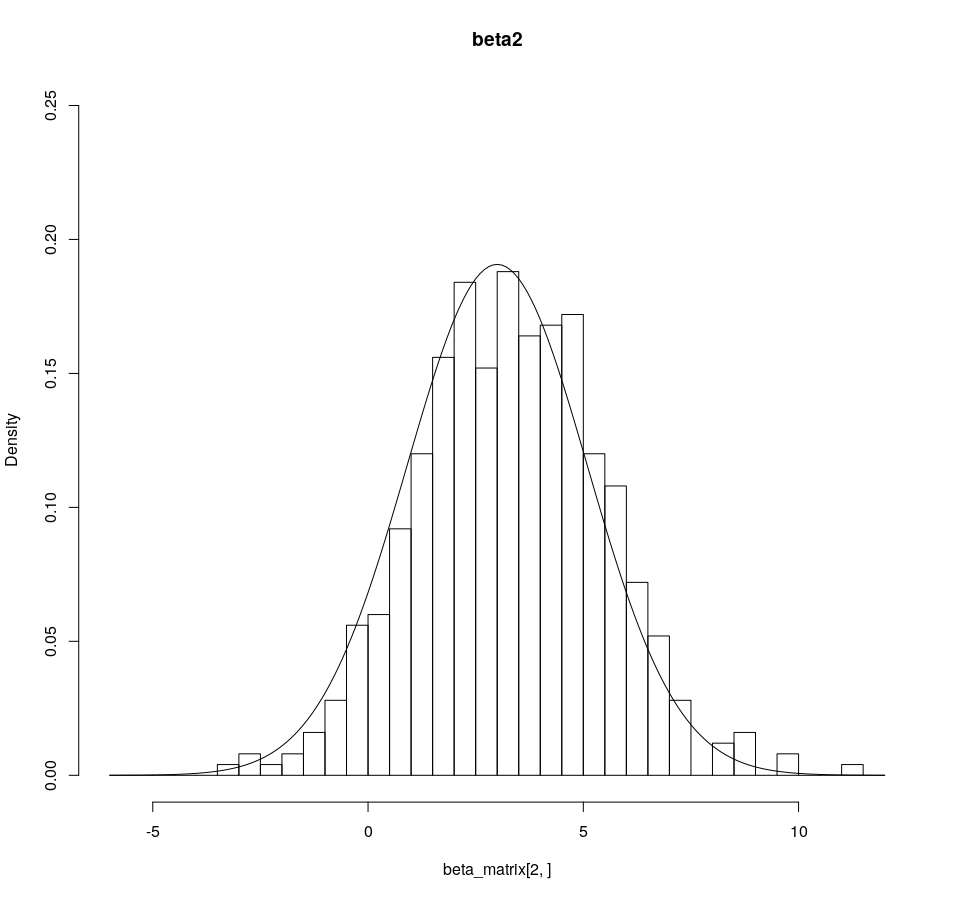
\includegraphics[scale=.35]{522.png} 
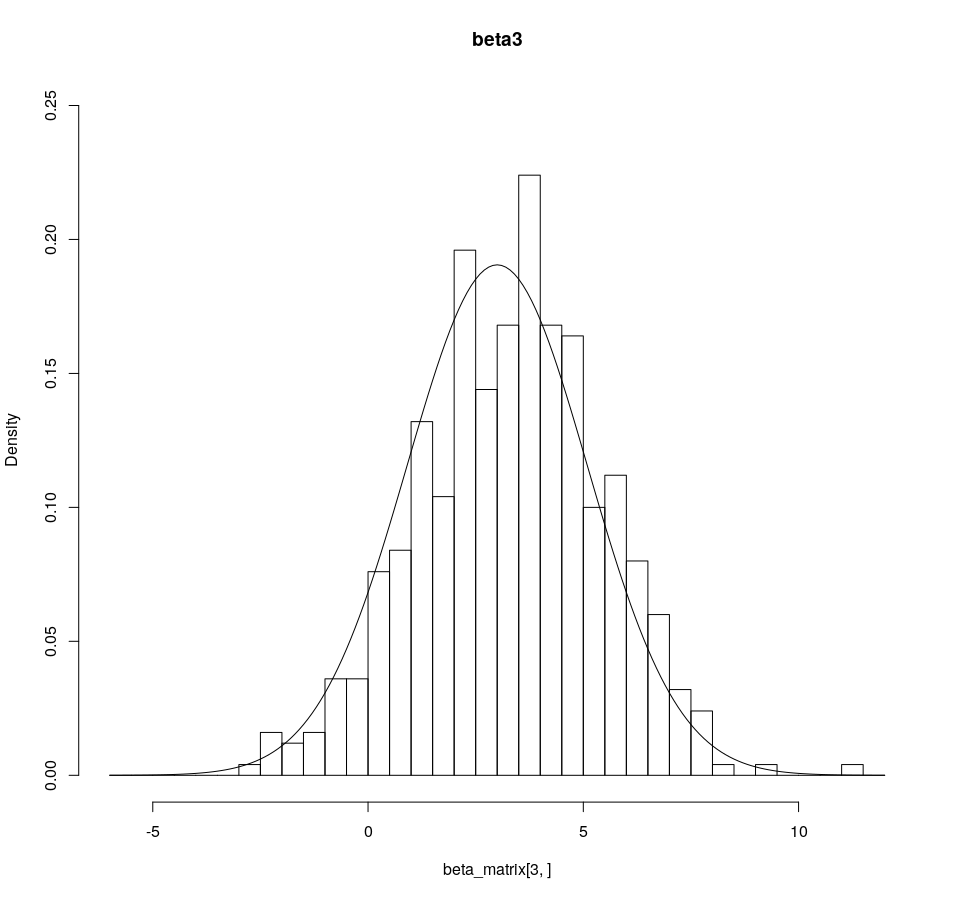
\includegraphics[scale=.35]{523.png} 
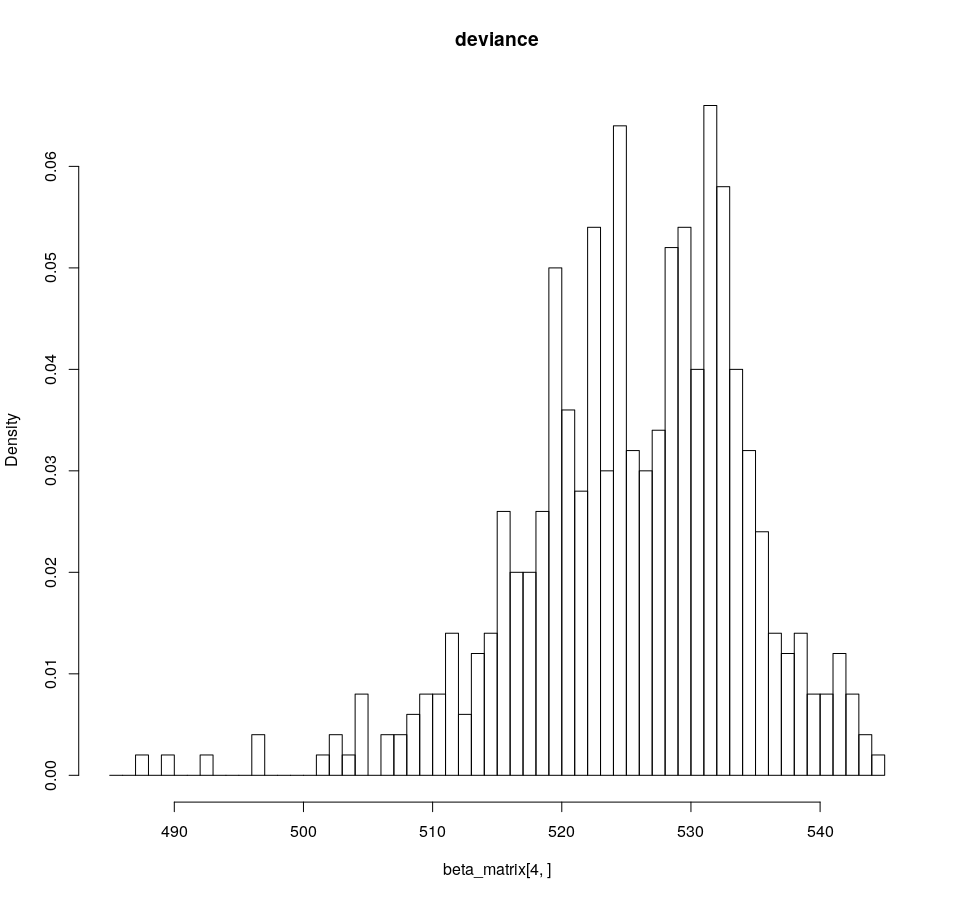
\includegraphics[scale=.35]{524.png} 



\paragraph{b} Obciążenia estymatorów $\widehat{\beta_{1, 2, 3}}$:

$

bias(b_{1}) = 0.163725

bias(b_{2}) = 0.2955454

bias(b_{3}) = 0.3109781$


\paragraph{c} 

Wyestymowana macierz kowariancji :

\left(\begin{array}{ccccccc}
1.122355e-02 & -0.007194674  &  0.004279991  &  7.857526e-05 &   0.01555513 &  -0.007613947 & \ldots \\
-7.194674e-03  &  4.889265050  & -0.250790032 &  -3.539216e-01  &  0.29441646  & -0.095619358 & \ldots \\
 4.279991e-03 &  -0.250790032 &   4.480899217  & -6.125341e-02 &  -0.19637423 &  -0.244461138 & \ldots \\
 7.857526e-05 &  -0.353921630 &  -0.061253410   & 4.475031e+00  & -0.10582805  & -0.257699219 & \ldots \\
 1.555513e-02   & 0.294416463  & -0.196374233  & -1.058280e-01   & 4.74489495  &  0.251669327 & \ldots \\
 -7.613947e-03  & -0.095619358  & -0.244461138 &  -2.576992e-01   & 0.25166933  &  4.273667462 & \ldots \\
 \dots & \dots & \dots & \dots & \dots & \dots & \ddots \\
\end{array}\right)

\subsection{n=100}


\paragraph{Macierz informacji Fishera} w puncie $\beta = (0, 3, 3, 3, 0, 0, 0, \ldots)'$:

\left(\begin{array}{ccccccc}
 23.37740799 &   2.001258e-01   & 0.0730452891 &  -0.1182702554  &  1.636312e-01 &  -0.127307567 & \ldots \\
 0.20012579  &  1.925539e-01   & 0.0244930108  &  0.0108764657  & -9.578576e-05  &  0.033875710 & \ldots \\
 0.07304529  &  2.449301e-02   & 0.3058456161   & 0.0002064384  & -4.111820e-02  & -0.014239494 & \ldots \\
-0.11827026  &  1.087647e-02   & 0.0002064384   & 0.1838149952   & 8.124780e-03   & 0.003642053 & \ldots \\
 0.16363119  & -9.578576e-05  & -0.0411182042   & 0.0081247801  &  2.062045e-01  & -0.018203970 & \ldots \\
 -0.12730757  &  3.387571e-02 &  -0.0142394937   & 0.0036420533 &  -1.820397e-02   & 0.274174406 & \ldots \\
 \dots & \dots & \dots & \dots & \dots & \dots & \ddots \\
\end{array}\right)

\paragraph{Macierz kowariancji} w puncie $\beta = (0, 3, 3, 3, 0, 0, 0, \ldots)'$:

\left(\begin{array}{ccccccc}
0.052120649  &  0.01119199  & -0.05506969 &   0.008541025 &  -0.04301242  &  0.03285469 & \ldots \\
 0.011191987  &  6.92120968  & -1.02118248  & -0.574051068 &  -0.07329602 &  -0.60041111 & \ldots \\
 -0.055069690 &  -1.02118248  &  4.18269753  &  0.341389399  &  0.79967576  &  0.20227475 & \ldots \\
 0.008541025  & -0.57405107  &  0.34138940  &  6.305626489  & -0.36044794  & -0.07965277 & \ldots \\
 -0.043012418  & -0.07329602  &  0.79967576  & -0.360447936  &  5.61290603  &  0.37125000 & \ldots \\
0.032854694  & -0.60041111 &   0.20227475  & -0.079652768  &  0.37125000  &  4.09708413 & \ldots \\
 \dots & \dots & \dots & \dots & \dots & \dots & \ddots \\
\end{array}\right)

\paragraph{a} Histogramy $\beta_{1, 2, 3}$ i deviance:

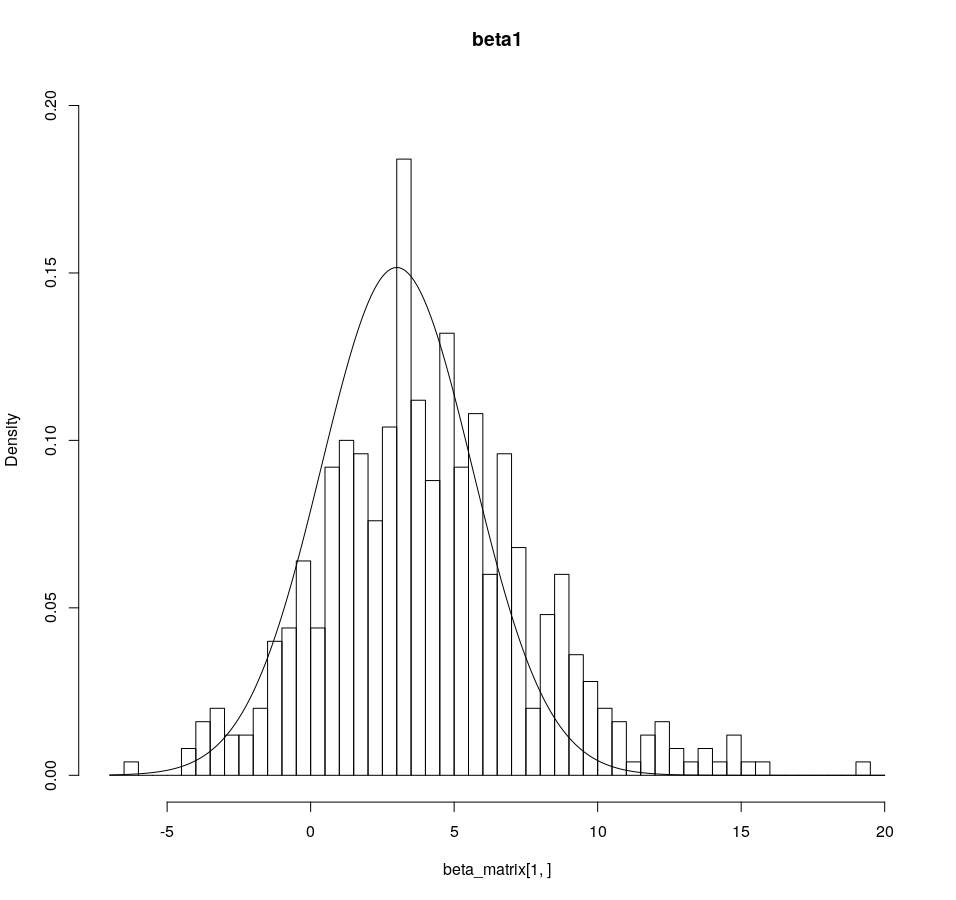
\includegraphics[scale=.35]{531.png} 
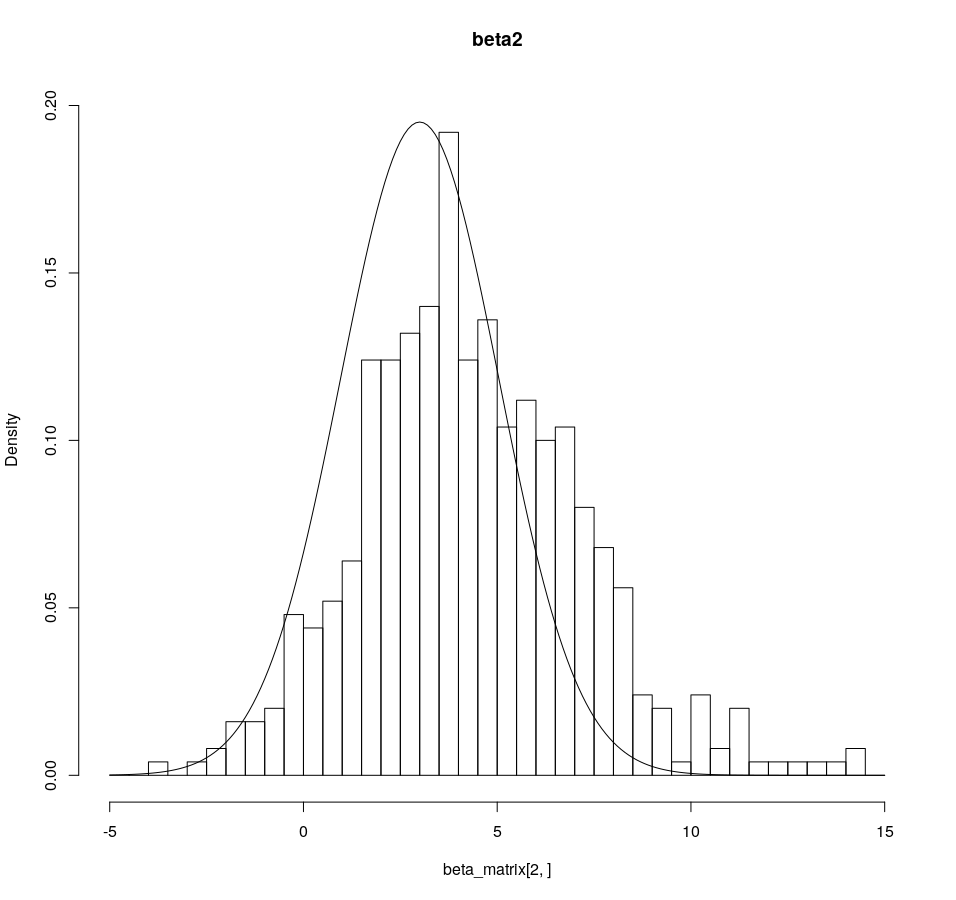
\includegraphics[scale=.35]{532.png} 
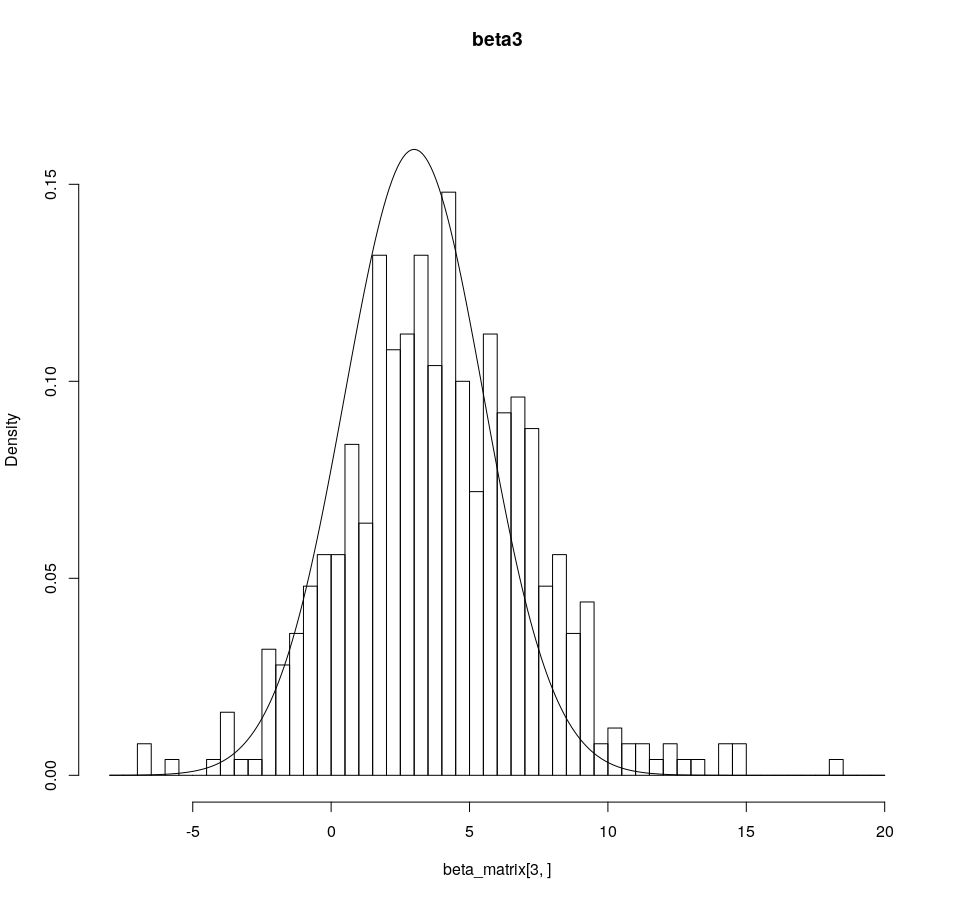
\includegraphics[scale=.35]{533.png} 
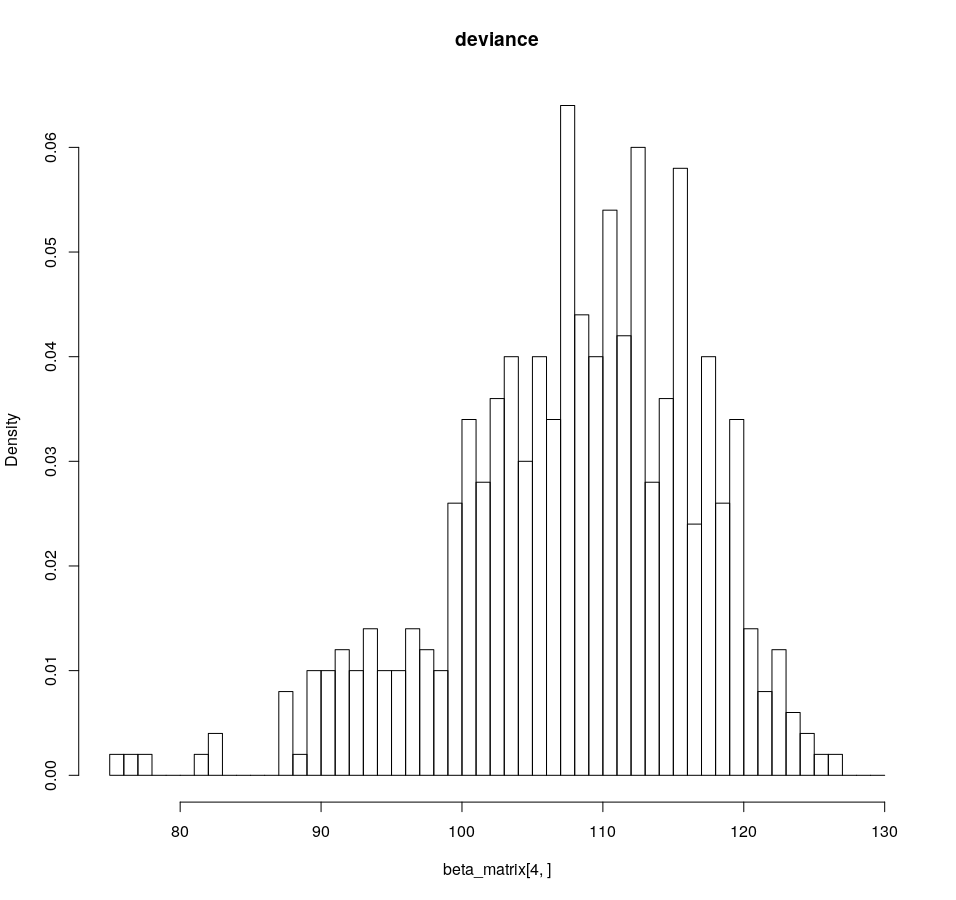
\includegraphics[scale=.35]{534.png} 


\paragraph{b} Obciążenia estymatorów $\widehat{\beta_{1, 2, 3}}$:

$

bias(b_{1}) = 1.119492

bias(b_{2}) = 1.329651

bias(b_{3}) = 0.9156808 $


\paragraph{c} 

Wyestymowana macierz kowariancji :

\left(\begin{array}{ccccccc}
 0.074450048 &  -0.007067676  & -0.1369618 &  -0.07468648 &  -0.009048333 &   0.04686173 & \ldots \\
-0.007067676  &  9.293511554  & -0.9682030  & -0.94835635  & -0.494283441 &  -0.99358031 & \ldots \\
-0.136961835  & -0.968203014   & 7.0442408  &  1.02462375  &  1.282408102  & -0.98789799 & \ldots \\
-0.074686479 &  -0.948356346  &  1.0246238  &  8.84023525  & -0.509839140  & -0.91046896 & \ldots \\
-0.009048333  & -0.494283441  &  1.2824081  & -0.50983914  &  7.445481563  &  0.36932106 & \ldots \\
 0.046861726  & -0.993580312  & -0.9878980  & -0.91046896 &   0.369321062  &  6.37651839 & \ldots \\
 \dots & \dots & \dots & \dots & \dots & \dots & \ddots \\
\end{array}\right)

\subsection{Wnioski:}

Przy zmianie n obserwujemy sytuację analogiczną co dla p=3. 

Zwiększenie p spowodowało większe zaszumienie. Przez co dla obu zadanych n wyniki okazały się słabsze niż w zadaniach 2 i 3. Są to błędy zauważalne, ale w zależności od sytuacji mogą się okazać akceptowalne (a także skłonić do poszukiwania lepszego modelu - o mniejszej ilości zmiennych objaśniających). 

\end{document}
